\chapter{The Instructor Perspective}
This chapter highlights the first study conducted regarding GitHub use in education. The study was conducted in collaboration with Alexey Zagalsky, Dr. Margaret-Anne Storey, Yiyun Zhao, and Weiliang Wang. My personal contributions include being a part of the data collection and interviewing educators, being involved in the coding process during the data analysis, and summarizing the findings and the discussion in collaboration with Alexey Zagalsky and Dr. Storey. \todo{I think you should come at this intro differently as I find it to be a bit too passive. It was way back in chap 1 that you introduced that you did two studies. I think you should reinforce that here...'As part of this work, we conducted two studies... This chapter highlights...' Or something along those lines (but much more thrilling!). I also wonder how much of this is verbatim from Alexey's paper...and given that you weren't first author, what are the implications of using this content in your thesis?} %need I be more specific?

\section{Research Questions}
We devised a number of research questions geared towards exploring the use of GitHub in education, a tool otherwise geared towards software developers. The research questions addressed in this study include:

\textbf{How does GitHub support learning and teaching?} We investigate how GitHub is used within the education domain and for what purposes. %Our findings indicate that even though GitHub use in education mirrors the way traditional learning systems are used, the implications differ substantially.

\textbf{What are the motivations and benefits of using GitHub for education?} Based on testimonials from our study participants, we explore the motivations for GitHub use in education and the possible benefits it might bring to support learning. We also look at specific GitHub features that are being used in this context.

\textbf{What challenges are related to the use of GitHub for education?} We examine the challenges educators and their students face when using GitHub to support learning and teaching. We provide specific examples based on interviews with educators, and later synthesize recommendations for educators wishing to use GitHub, as well as recommendations to the GitHub design team.

\section{Research Design}
In the first phase of our study, we used online research methods \cite{wakeford2008fieldnotes} and searched for resources (such as blog posts) that described the personal experiences of educators using GitHub to support learning or teaching. The results from this phase are presented in the Background section.\todo{This wasn't clear to me. I don't recall you pointing this out in that chapter.} Through this exploratory phase, we found creative and successful examples of GitHub supporting teaching and learning in the classroom. We also found discussions on the challenges and difficulties of using GitHub. This allowed us to refine our research questions and guided us in the following phases of the study, such as shaping the questions to ask during interviews.

In the second phase of our study, we interviewed 15 participants, including a blog author we discovered in the first phase. Here we were able to thoroughly investigate the usefulness and potential of GitHub in education. Through iterative analysis of the data collected, several themes emerged around the motivations for and challenges of using GitHub to support learning. These themes informed the third phase of our research: a follow-up survey sent to interviewees from the second phase and to other educators using GitHub for education. The goal of this survey was to receive interviewee feedback on our interpretations, but also to gain additional perspectives from other educators that use GitHub.

\subsection{Participants}
Our study targeted lecturers and professors in higher education who use or have used GitHub to support teaching and learning. As our study aimed to investigate diverse populations as well as GitHub's usefulness in non-technical courses, we wanted to hear from lecturers and professors across domains.

\subsubsection{Interview Participants}
Table \ref{table:interviews:github_tutorial} shows some details about the courses each of the interviewees taught using GitHub. For each course taught, we list a summary of the students' GitHub knowledge, the type of course, and the number of students enrolled.

\begin{table}[h]
    \vspace{1pt}
        \caption{Information on courses taught by interview participants while using GitHub.}\label{table:interviews:github_tutorial}
    \vspace{1pt}
    \begin{center}
        \begin{tabular}{cccc}
            \hline
            P\# & \multicolumn{1}{|c}{Course Type} & \multicolumn{1}{|c}{Knew GitHub} & \multicolumn{1}{|c}{Course Size(s)} \\
            \hline
            1 & CS & Yes & ~55 \\
            2 & CS & Yes & ~40 \\
            3 & CS & Yes & 85, 130 \\
            4 & Humanities & No & 11, 40 \\
            5 & Humanities & No & 17 \\
            6 & CS & Yes & 60, 100 \\
            7 & CS & Yes & 50-237 \\
            8 & CS & Varies & ~60 \\
            9 & Sciences & No & 235 \\
            10 & CS & Varies & 450 \\
            11 & CS & Varies & 20, 40 \\
            12 & Statistics & No & ~40 \\
            13 & CS & No & 20 \\
            14 & CS & Yes & 8 \\
            15 & CS & No & 30-32
        \end{tabular}
    \end{center}
\end{table}
The participants represent a broad list of universities: University of Victoria, University of British Colombia, McGill University, University of California at Berkeley, University of California at Davis, Columbia University, The City University of New York, Harvard University, The University of Texas at Austin, Federal University of Pernambuco, and Delft University of Technology. Furthermore, one of the participants was from a company that teaches code to entrepreneurs and CEOs in Paris.

\subsubsection{Follow-up Survey Respondents}
We sent a follow-up survey to the interviewees to get their feedback on our interpretation of the interview findings. We also publicly broadcasted the survey using social media\footnote{\url{https://twitter.com/alexeyzagalsky/status/471053256718692352}} and used snowball sampling to garner responses from additional educators. Eight of the interview participants and an additional seven new respondents completed the survey, for a total of fifteen responses.

\subsection{Data Collection}
For the interviews, we emailed invitations to lecturers and professors that use or have used GitHub to support teaching or learning. Potential participants were recruited in several ways: by contacting blog authors who shared their experiences of using GitHub in the classroom; by posting an invitation on Twitter\footnote{\url{https://twitter.com/alexeyzagalsky/status/465914075348619264}}; and through snowball sampling, where interviewees could suggest other colleagues.

The interviews lasted 20-60 minutes and were conducted face to face or with Skype. Audio was recorded and the interviewer took notes. The interviews were semi-structured based on 18 guiding questions (our interview form is available in Appendix A), and the interviewer \textit{dug deeper} with additional questions as deemed appropriate. This supported the exploratory nature of our study and allowed us to examine interesting and unexpected insights.

We also interviewed John Britton, an education liaison from GitHub (this interview form is also available in Appendix A). This interview provided us with GitHub's corporate take on the use of its tool in education.

\subsection{Data Analysis}
Our analysis of the interview data followed qualitative data analysis guidelines \cite{lacey2001qualitative,seaman1999qualitative} and included the following stages: (1) transcription of the data recorded; (2) organization of the data into easily retrievable sections; (3) familiarization by reading and re-reading the data, making memos and summaries; (4) reading the data and labeling segments, i.e., coding; and (5) identifying themes or emergent concepts through discussions among the researchers and engaging in re-coding to develop more well-defined categories. After refining and merging some of the themes, a list was compiled. This process was performed iteratively for each category.

\section{Findings}
\label{sec:results}
In this section, we address our research questions and present the themes that emerged from the interviews. To illustrate the different aspects of each theme, we provide selected quotes from the interviews, where each participant is identified by an anonymized identifier (P\#).

\subsection{RQ1: How does GitHub support learning and teaching?}
There are two ways that our interviewees utilized GitHub in the classroom: as a submission platform, and as a way to host course content. These two basic uses mirror how teachers use typical Learning Management Systems (e.g., Moodle and Sakai) \cite{malikowski2007model}. However, the implications of how they use these features differ substantially. Figure \ref{fig:edu_workflow} gives a high-level overview of the interactions that are possible between teachers, students and content, and shows the additional interactions that the use of GitHub natively supports over traditional learning environments. For example, as seen in the bottom-left quadrant of the figure, while traditional LMSs support students reading and accessing course material, GitHub also allows them to easily contribute to the course material.

\begin{figure}[h!]
 \caption{The additional features GitHub provides in addition to the features provided by traditional LMSs.}
 \centering
   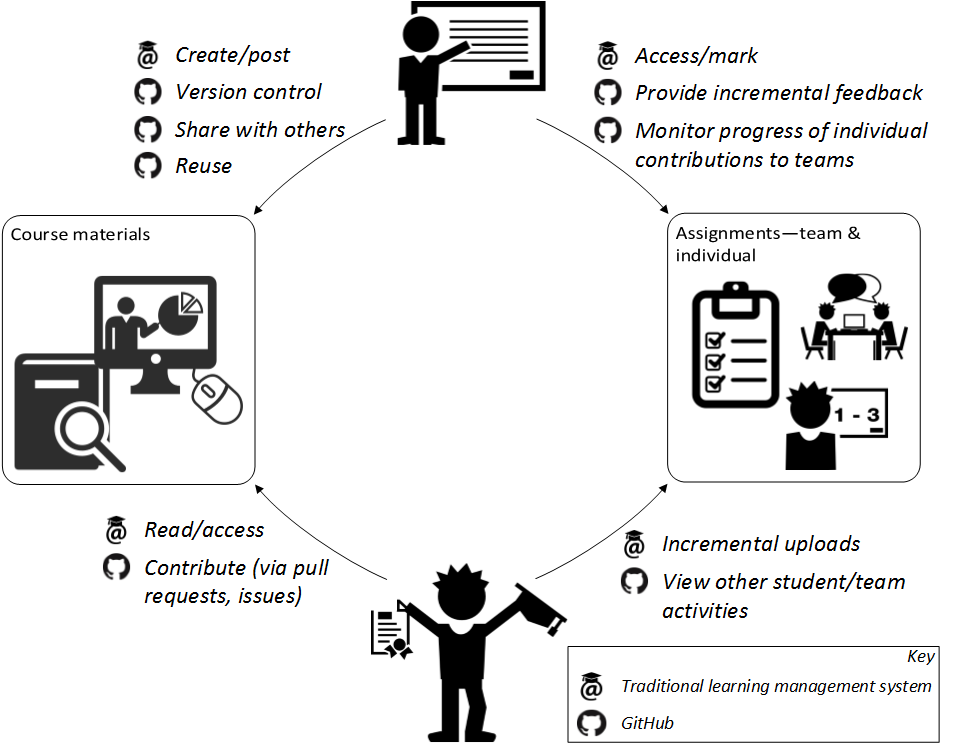
\includegraphics[width=0.8\textwidth]{EduWorkflowLargeType}
 \label{fig:edu_workflow}
\end{figure}

\subsubsection{GitHub as a Submission Platform}
Many of the interviewees used GitHub as a place for students to host their work and submit their course assignments and projects, \textsubscript{P1, P2, P3, P4, P5, P6, P7, P11, P12, P13, P14, P15}. The benefits of using it as a submission platform are further discussed in the findings of RQ2.

Using GitHub as a submission platform was accomplished in one of two ways\footnote{\url{https://education.github.com/guide\#4-set-up-the-repositories}}. Some interviewees set up a base repository for the class and had each student fork it---everyone who forked the base repository could see all other forked repositories as well. This allowed students to cross-reference different solutions and encouraged student collaboration (e.g., by using PRs) and peer learning. \textit{``When you do a pull, you can see what the others in the seminar are doing. For example, a student wrote a python script, and others want to use it, so they can just grab it and use it.''}[P4]

Other interviewees set up private repositories for each student, and individual students could only see other repositories when explicitly given access. For P5's course, \textit{``Students have separate repositories, and it's private so that people cannot see what they are working on.''} With this option, repositories and permissions are manually configured, which may be difficult in courses with a large number of students.

\subsubsection{Hosting Course Material}
Many interviewees used GitHub to host and deliver course materials \textsubscript{P4, P5, P8, P9, P10, P11, P12, P13, P15}, including syllabi, slides, notes, reading materials, exercises and homework. It was even used to host the actual course Website, making GitHub \textit{``a bulletin board.''}[P10] The basic mechanism to host course Websites is by using GitHub markdown files, or for more traditional Websites, by using GitHub Pages\footnote{\url{https://pages.github.com/}} to host the material directly from one's repository.

With course materials hosted on GitHub, students and other educators were able to suggest course improvements [P1, P10, P11, P12] by submitting an issue or a PR. \textit{``Students would actually find corrections and things and they would send me pull requests... But there was some sense of a community that was at least, certainly invited to collaborate on the course material itself.''}[P12] As such, interviewees were able to facilitate student contribution to the course material itself using GitHub, a use case and benefit that GitHub offers beyond many traditional systems.

\subsection{RQ2: What are the motivations and benefits of using GitHub for education?}

We explored why educators chose to use GitHub and how they (and their students) benefited from its use. While GitHub is still an emerging tool for education and many benefits have not yet been fully realized, we extracted several themes from our interviews.

\subsubsection{Transparency of Activity}
Using GitHub as a submission platform made it easy for our interviewees to monitor student progress, activity and participation. GitHub has numerous features that support transparency. For example, GitHub allows users to see the \textbf{history} of activities. As P1 mentioned, \textit{``You really see the full history of how the document comes into being, including all the discussions, the former versions. And the groups can look at each others' documents and see them emerge. I can see how they are creating it, so I can monitor who's active, working in certain teams, which is also handy, practical.''}

GitHub also provides a \textbf{graph view} that visualizes a summary of project activities. This allowed teachers to easily gain a high-level view of student activity. \textit{``You can see who is doing what, you can see how people are sharing work because you have the commit history.''}[P4] This same feature supported teachers in identifying students that were not participating as expected. \textit{``I would go into their team repository, and...they have some graphs in there that show you what's the activity level and who's most active. I would use that to get a sense for what was happening because inevitably, you would have one of the students...that's not doing anything and you want to get some hard data on exactly what he isn't doing.''}[P6]

Furthermore, GitHub has a \textbf{News Feed} that teachers used to keep up to date with activity. By watching the News Feed, they could catch problems early and saw how frequently students were participating in the course. \textit{``Personally, what I did is that I subscribed to all [the students'] repositories and followed the feed of those repositories.''}[P2]

However, GitHub allowed people to do more than just passively observe progress. Students \textbf{opened issues} and \textbf{tagged} them with the teacher's name to get their attention. \textit{``You could watch the commits go by. They can ask for help by opening issues and tagging us, so that worked quite beautifully for monitoring and in some cases actively providing advice on group project work.''}[P12] This kind of support encouraged a style of communication between the teacher and student that is not available in traditional Learning Management Systems.

\subsubsection{Encourage Participation}
The transparency features discussed above allowed interviewees to encourage student course participation and contribution to the hosted course materials. With traditional environments, students would need to contact the instructor directly to suggest changes to the materials. Using GitHub, a student could suggest changes by submitting an issue connected with the material. Or, they could make changes themselves and then submit a pull request which the teacher, if they agreed with the changes, could simply accept. The history of these actions helped the teacher keep track of who participated, and by its visibility, also encouraged students as their actions were logged and possibly used to improve their grades.

P1 spoke about how these features helped to persist the effort that students put forth:
\textit{``Yes, [using GitHub encouraged student participation] because everything you do is also recorded. It stays there forever, it's persistent. So your comments are persistent, your activities are persistent. So you work, you get rewarded, and if you don't work it's visible... in GitHub it's a little more transparent.''}

Some interviewees felt that using GitHub helped them encourage participation, even in indirect ways: \textit{``I will use the logs [that students put on GitHub] as materials for discussion in class. That can encourage participation because you know you are committing something that can be discussion material.''}[P5]

Although few mandated the use of GitHub's issue tracker for their classes and group projects, some found novel uses for this feature. P12 and P14 had students use it when they needed help, and otherwise used it as a simple communication method between students and markers. P1's students participated by discussing an issue they had with a deadline: \textit{``the students didn't like [a deadline], so they opened an issue on GitHub: `Can we move it?'... So everyone responded to that issue on GitHub, and then at the end I said, `based on the discussion, it is going to be on Sunday.'''} These features supported student/teacher discussions---communication was recorded and tied directly to the relevant course content.

\subsubsection{Reuse and Sharing of Course Materials and Knowledge}

Another important advantage GitHub provided our interviewees was the ease with which materials and knowledge could be shared and reused, by both students and course instructors.

Some of our interviewees' students shared work and materials with each other. In P4's course, a student's python script was visible to others, and therefore, easily shared. The ability to make content either public, private amongst collaborators, or completely private, gave our interviewees' students an easy way to share with others or contribute to their work. For example, P1 noted that this visibility had the useful side effect that his students gave each other \textbf{feedback} on their pull requests and reports.

Moreover, our interviewees used GitHub to share courses and their associated materials with other educators. Although this is also a feature in many learning environments, they lack a way to visualize how a reused course has changed from the original content. Seeing when courses are \textbf{forked} and how they differ from one another is a key feature in GitHub.
\textit{``We were developing all the content from scratch... the various teaching staff had to collaborate and develop the material, and so GitHub was a nice fit for that... We had two repositories: we had a private one and a public one, and so we could sort of have private conversations among the staff to refine the content and then it was pretty easy to just migrate it over once it was ready.''}[P10]

GitHub's \textbf{access control} features allowed the instructors to \textbf{version} their material and choose whom to share it with. \textit{``Some of [the material] is shared with the world, and some of it is shared with other instructors of other universities. So for example, when we create new exam questions and stuff like that, we try to keep those [repositories] private for a little while so other instructors can use them. But we're versioning all of it.''}[P7]

Interestingly, unregistered students and other GitHub users would also visit these public repositories: \textit{``We kept everything public from the beginning, so it ended up getting a lot of attention outside of the course. I think the repository has something like 200 stars on GitHub right now and as far as I can tell most of those stars are from people who didn't take the course.''}[P10]

\subsubsection{Industry Relevance}
As working with Git and GitHub are relevant skills for industry, this theme emerged as both a motivation to use GitHub in courses and a benefit of using the tool. This relevance to industry meant that some of our interviewees and their students had prior GitHub experience, and as a result, were motivated to use it in class. For example, P12 had already been using GitHub regularly and explained why they chose to use GitHub in their courses: \textit{``... partially to unify what I'm doing in the research side of my life with what I do with the teaching side. Like once you've taken the trouble to learn [GitHub] and get it all set up, you start to see lots of areas of your life where this workflow would actually be very useful.''}

Meanwhile, we saw some instances where students who had prior experience using GitHub encouraged their course instructors to use it for class. As P1 told us: \textit{``So actually, some students came to me, and they said: you should watch this video on how GitHub uses GitHub to build GitHub.''}

Knowing how to use Git and GitHub is a significant benefit in certain fields, particularly in computer science and software engineering [footnote]. In fact, P12 felt that learning to use GitHub was required to progress within their field: \textit{``To prepare this cohort of graduate students for computational work, they should know how to use these tools. This is very much what people do these days in [statistics], and so I actually consider it a completely valid pedagogical goal in it of itself.''}
%\url{http://techcrunch.com/2014/07/23/modernizing-computer-science-education}

By using GitHub for course work, students further benefited by having an end product that could easily be shared with prospective employers. \textit{``you can use it sort of as an online resume... GitHub allowed you the opportunity to convert [your class work] to a public project so that employers for example could see what code you've been writing.''}[P6]

\subsubsection{Ease of Use}
GitHub's administrative functions are relatively simple and easy to work with: getting students set up for the class, setting privacy options, and creating repositories. \textit{``I don't think it saved time at the beginning... because I was starting an entirely new approach to doing this. But once it was up and running, the next semester would have been quite simple to administer because I knew the process.''}[P6] Although GitHub has a definite learning curve, it can be mitigated by sharing practices among practitioners. \textit{``I worked with [the next instructor of the course] a bit on explaining how it worked and what we did with it, so she found it pretty easy to get started too.''}[P6]

Despite the learning curve and some technical difficulties, several interviewees mentioned that GitHub was relatively easy to use and administer, both on its own and compared to existing university systems. \textit{``For me it was the ease of updating the class schedule and course notes. The class schedule is something that is extremely painful to update on the university Website... Each course is a little window and you have to click arrows to move them up and down to reorder them, or something really horrible like that. And [with GitHub] it was very easy to just go into a markdown, add a link, and hit push.''}[P9]

\subsubsection{Free Academic Licenses}

Generally, GitHub allows all users to create free public repositories. However, an additional benefit mentioned in the interviews [P3, P6, P7] is that GitHub provides free academic licenses. Students and educators can apply for a free micro plan that allows private repositories. Educators can also apply for a free organization account [footnote] that facilitates team management and administration. The implications of these free public accounts go beyond benefiting face-to-face instruction, allowing teachers to \textit{scale-up} traditional education and create online courses that will benefit part-time and remote students.
%\url{https://help.github.com/articles/what-s-the-difference-between-user-and-organization-accounts}

\subsubsection{Shared Space and Course Versioning}
By hosting course materials on GitHub, students could easily share course notes, references or other material for the same class, and educators could quickly share [P13] or duplicate course resources. \textit{``The simplest thing I've been using [GitHub for], especially from an instructor's view, is to duplicate the course Website for different semesters.''}[P4] Therefore, when teaching the same course again, preparing the course materials was simple: participants used the same repository or forked it. \textit{``If I improve the material in some way, I'd just keep it there...And if someone wants an older version of the repository, they just need to get it. However, if I did want to create a separate course with just part of the material of the original course, I would [fork the repository].''}[P11]

\subsection{RQ3: What challenges are related to the use of GitHub for education?}
We have grouped the challenges our analysis revealed into five themes: shared knowledge base of suggested practices, barriers to entry, support for additional formats, external restrictions, and large-scale management.

\subsubsection{Shared Knowledge Base of Suggested Practices}
Interviewees showed a need for \textit{a shared knowledge base} of suggested practices on how to use GitHub for educational purposes. P6 went into great detail about their struggles in this area: \textit{``It's a different use in a team at some startup or what have you. And it's not clear how exactly you should, for example, enforce a methodology for the students for working. Should you use pull requests? When should you file issues? Divide up the repository, should you each have an individual repository as well and then fork the main project? There's a lot of good evidence and good data for how you should work in Git for your software development project, for commercial projects. For educational projects, they're quite different because they're short in duration, there's 4 or 5 people working on it that aren't very experienced with software development.''}

Educators wished for easily accessible \textit{how-to guides} or shared experiences by others who have used GitHub. \textit{``Maybe some documentation on best practices or some kind of shared knowledge base that would say here's what so-and-so at UC Irvine is doing with GitHub.''}[P6]
Interestingly, the GitHub education Website contains a guide that could meet some basic needs, but our interviewees did not know of this relatively new feature.


\subsubsection{Barriers to Entry}
At its core, GitHub is a \textbf{Git-based} system, and while it provides a simple Web interface, tasks that involve collaboration require an understanding of Git and its command-line arguments. In particular, dealing with \textbf{merges and conflicts} can be challenging: \textit{``To get the most out of GitHub, you need to understand Git. Even if you just use it to edit documents together, you will get conflicts once in a while. And if you want to use the review mechanism, then you want/should use the pull requests. That requires some pretty deep knowledge of Git still. If you use it the right way it is simple, but somehow with Git you end up with conflicts, and if you don't understand it, it's magic.''}[P1]

Difficulties using Git are experienced by technical novices and software developers alike \cite{perez2013s}. Our interviewees reinforced the need to improve \textbf{accessibility} for novice users or users with a limited technical background: \textit{``Largely, the biggest challenge is to lower the learning curve, not on the high end, but the very low end for people who are new to it to have much gentler learning curve.''}[P5]

\subsubsection{Support for Additional Formats}
GitHub's file and format support is another main challenge mentioned by the interviewees, specifically the lack of support for formats widely used in education, such as PDF and LaTeX. The ability to view or render these formats directly on GitHub, similar to Markdown rendering, would be very helpful. But more importantly, there is a need to support the powerful features Git has for text files: \textit{diff} and review functionality, and the mechanism to add inline comments to a file without altering the original file. For example, when an instructor wishes to mark the students' assignments or reports, they are forced to download and comment on each file separately (e.g., using the comment feature in a PDF file), which also alters the original file. Another option is to use the \textit{issues} mechanism of GitHub to provide comments, however, this mechanism can't reference a specific place in the file and may be tedious if the instructor wants to add many small comments to a submission.

Interviewees also mentioned GitHub's poor support for slides: \textit{``You can not easily view slides in GitHub, because the PDF is too large and you have to download it, it's a bit cumbersome... in a course you always have presentation material, so you want some sort of integration with slides here. They [GitHub] have Speaker Deck, so I want Speaker Deck integrated with GitHub.''}[P1] Being able to \textit{diff} slides would be highly beneficial.

\subsubsection{External Restrictions}
Interviewees also mentioned external restrictions that limit or prevent them from using GitHub for education. External restrictions can be local restrictions (e.g., university policy) or global restrictions (e.g., regional publishing licenses). \textit{``We have LMS systems that we use, and in a way it's very important to use them because they're authenticated by the university. So things like student's grades and stuff like that you don't (store on GitHub), because of the rules in the US. You cannot store it anywhere else.''}[P3]
Another teacher also shared this concern:
\textit{``Ethically, I wish I could know where the server is, where I am pushing all my material.''}[P4]

Knowing the server's location plays a significant role when educators decide whether to use GitHub. Not only from the \textbf{ethical aspects}, but also for \textbf{copyright reasons}. As P5 mentioned: \textit{``Copyright is a big issue. For instance, we are working with a novel. In Canada, that novel is in public domain so it can be accessed online, but not in the United States.''}

\subsubsection{Large-scale Management}
Educators are challenged when managing courses with large numbers of students, teams, projects or issues. \textit{``One thing I'm not so happy with, is the way group management [works]. So managing teams, different sizes, I have an organization for the students and the organization has 50 members and I need to create different groups, and different roles, and different access... I think that could be done... [in a] more convenient way.''}[P1]

P6 further discusses the challenges with managing teams and repositories: \textit{``The thing that I think was missing... was more management for the administrator: assigning people to teams, assigning teams to repositories, finer grained permission control, I think [that] is something that could have been useful.''} However, the cause of these difficulties might not be an issue with GitHub, but perhaps the lack of \textit{how-to guides} and suggested practices by others.

\subsection{GitHub's Perspective}
To gain insights into GitHub's perspective on the topic, we interviewed John Britton, an education liaison at GitHub and one of two engineers working full time to support the use of GitHub in education. GitHub's main goal in this regard is to make the tool easier to use, and to make sure users are aware of what resources are available to them to meet their needs and solve their challenges. \todo{I don't like the use of these quotes without much supporting content (words) of your own. You should summarize like with all the quotes above.}

Regarding GitHub's benefits for education, John replied:
\begin{quote}\textit{``We're working with students and teachers on using GitHub. It's essentially leveraging those tools in the classroom, so you can get a classroom experience that's more similar to what people in the industry are using, as software developers.''}\end{quote}

However, there are challenges involved:
\begin{quote}\textit{``When I first started, I definitely was targeting all forms of education. But I think that it's most applicable in computer science, software engineering, and technical fields. Maybe someday when the tools are easier to use and... require less technical knowledge upfront, it will be much more useful to non-technical fields, or to other types of educational stuff. But I think that Git as it stands requires a certain amount of basic knowledge of computing.''}\end{quote}

He then elaborated:
\begin{quote}\textit{``There's different groups. People who know Git and GitHub already and just want to use it in the classroom---they're totally on board with using pull requests right from the beginning. The group of people who's like, `What's Git? What's GitHub?', they have a little bit harder time getting into the mindset of students submitting their code as a pull request. Rather than submitting an assignment with a zip file, you create a branch and make a pull request, and then grade the student on the pull request''}\end{quote}

John concluded by describing how GitHub plans to assist educators:
\begin{quote}\textit{``I think we're going to do more of those [stories of existing use cases], along with technical documentation, or technical information on `Here's what they're doing. Here's how you can do it too'. But as far as...we don't have a set, like, this is the way, right? There are multiple ways to use GitHub in the classroom, and it depends on what goal you're trying to achieve.''}\end{quote}

The education use case is important for GitHub. While their focus remains on its use in software development, they provide dedicated support and resources for educators to take advantage of the tool.

\subsection{Follow-up Survey}
After conducting the interviews, we sent a follow-up survey to both interviewees and the public. We wanted to see if respondents agreed with our interpretation of the interview findings. However, the number of respondents (15) was too low to confidently validate our study. Regardless, the survey supports many of our findings, with respondents mostly agreeing or strongly agreeing to many of the uses (as a submission platform and course material host) and benefits (simpler than current university systems, reuse and sharing of material, and facilitating collaboration). Interestingly, many respondents from this group of educators stated that they didn't struggle with the challenges that emerged in our interviews (e.g., technical difficulties limiting educator GitHub use, external restrictions, and managing large groups). However, while strongly disagreeing that technical difficulties limited their own use of GitHub, most respondents agreed that technical difficulties limited their students' use of GitHub.

\section{Validation}
\label{sec:validation survey}
In the previous section, we described the emerging themes from the interviews. In this section, we describe the survey intended to validate our findings. This survey elicited responses from all who use GitHub for teaching purposes, including the participants interviewed. The survey received responses from professors and lecturers who have taught a variety of class sizes, from 6 to 200. Of the 13 respondents, 7 of them were those previously interviewed.

%some graphs here might be nice

\subsection{RQ1: Uses in Teaching and Learning}
The variety of uses highlighted in the sections above were confirmed by the respondents to our survey. 11 of the 13 respondents agreed with GitHub's use as a submission platform, more so with team projects (9) than individual student assignments (6). This seems to be the most common use of GitHub, as reflected in our interviews. Many of the respondents agreed with the use of GitHub to host the materials for their courses (11/13), and those that agreed primarily hosted course notes (7) or slides (7), reading material (9), and assignments. This asserts that GitHub can be an effective method of delivering a variety of course content.

%I added one of the benefits here because it seemed relevant
A majority of the respondents (8) used GitHub to monitor student activity and progress. A similar number provided feedback to their students using GitHub's features (7), while the same number shared teaching materials with other educators (7). Almost all agreed that an important benefit was the ability to reuse and share teaching material and knowledge (11). This suggests that many of the respondents used GitHub in such a manner, being able to reuse their own or others' materials. Approximately half of the respondents had their students use GitHub to suggest improvements to course materials (6).

It's possible that more educators would have utilized these features had they known how to use GitHub in such a manner. This is reflected by many respondents either agreeing or strongly agreeing (9) that they would appreciate having access to a knowledge base of shared practices on how to use GitHub for education.

\subsection{RQ2: Motivation and Benefits}
%needs graphs?
Our second research question asks why instructors are motivated to use GitHub for classes and what the benefits are. Respondents agreed or strongly agreed (9) that students should be familiar with GitHub on a professional level, and therefore, this motivated them to use it in their classes. However, this likely applies more to technical courses than non-technical courses.

Half the respondents agreed that GitHub allowed for transparency of activities among students (7), with about the same agreeing that GitHub helped them evaluate student performance (7), suggesting how beneficial it is to easily monitor activities performed in GitHub. As well, there was agreement that using GitHub facilitates collaboration, discussion, and participation among students (8), suggesting how useful it is as a collaboration platform.

\subsection{RQ3: Challenges and Difficulties}
Interestingly, most of the respondents disagreed or were neutral in their feelings that the technical support provided by GitHub motivated their use of the tool (8). Perhaps they didn't know how much support is available or they possibly felt that it was easy enough to use without technical support. Indeed, many respondents agreed that GitHub is easier to work with than the other systems used at their institutions (9). This is supported by most of the respondents disagreeing that technical difficulties were a challenge for them (8), however, when asked if difficulties experienced by their students limited their use of GitHub, more respondents agreed (6) than disagreed (4). This suggests that their students may have had a more difficult time using it than the instructors themselves.

Furthermore, external restrictions and managing large numbers of students or projects was not a challenge for most respondents (9). On the other hand, several respondents mentioned that they struggled with privacy concerns (5). And finally, most of the respondents (9) would appreciate having access to a knowledge base of shared practices on how to use GitHub for education. \todo{You already stated this above...perhaps rephrase/elaborate so it seems more meaningful?}

\section{Discussion}
Our study uncovered how some educators use GitHub to support learning and teaching, while extending or even replacing traditional LMSs. However, the implications of our findings go beyond GitHub itself. The emergence of \textit{``the GitHub way''} within education is transforming the traditional e-learning model, as seen in figure \ref{fig:edu_workflow}, and will better support socio-collaborative learning environments \cite{kreijns2002sociability} of the future.
%\ref{fig:edu_workflow}

\subsection{Comparing GitHub to Traditional LMSs}
GitHub was not designed as an LMS or a CMS\todo{Have you defined CMS previously?}, but our study shows it can be used as such. Judging the use of Git and GitHub based on LMS features \cite{kumar2011comparative}, GitHub supports many of the important learning components (e.g., assignment delivery and submission), but it also lacks certain features (e.g., grading management tools). In examining the model published by Malikowski \textit{et al.} \cite{malikowski2007model}, we come to similar conclusions, where platforms like GitHub have the capability to support all five categories of the model. However, student and course evaluation may require additional work, as well as developing programs to detect and automatically grade student pushes.

Lane \cite{lane2008toolbox} discusses two sides of the CMS. From one side, CMS are a \textbf{toolbox} for educators, providing a default course structure with managerial and administrative features. From the other side, integrated commercial CMS are a \textbf{trap} that limit faculty creativity, are difficult to customize (sometimes this involves additional cost), and they make it hard to accommodate individual teaching styles. As GitHub is adopted for more and more courses, it remains to be seen if it suffers from similar or different issues to mainstream CMSs.

\subsection{Going Beyond Traditional LMSs}
Beyond the features discussed above, GitHub provides a number of other tools and features that allow educators more novel possibilities.

\subsubsection{Version Control}
According to the interviewees that teach technical courses (such as computer science), students destined for careers in software and information technology benefit from learning to use version control systems \cite{britton2013using}. This reflects the benefits mentioned in previous work on these types of systems \cite{reid2005learning}. At the same time, version control allows educators to see the final results as well as the processes students used to produce the results \cite{glassy2006using}. However, this is a double-edged sword as the technical aspects of version control, specifically Git, is one of the main challenges mentioned by interviewees.


\subsubsection{Transparency \& Awareness}
Kreijns \textit{et al.} \cite{kreijns2013social} discuss the shortcomings of contemporary CSCL\todo{again, is this already defined?}, particularly in group learning, social construction of knowledge, and the learning process itself. They link these problems to the impeded social interaction of CSCL environments caused by two major pitfalls: taking social interaction in groups for granted, and the lack of attention paid to the social psychological dimension of social interaction outside of the task context. \textbf{Transparency of activities} allows GitHub to address this by embedding \textbf{social affordances} and by supporting \textbf{group awareness}, as proposed by the suggested theoretical framework \cite{kreijns2002sociability}.

However, only a few of our participants mentioned using the \textbf{transparency} and \textbf{awareness} features to promote collaboration among students. If taken advantage of, GitHub's transparency could be beneficial for collaborating students \cite{dalsgaard2009transparency}, creating awareness of each others' activities that could, in turn, support collaborator creativity \cite{farooq2007supporting}. As such, GitHub is a good example of a transition from a space to a place, as it transitioned from a hosting service that provided space for projects, to a place where work, activities, ideas and discussion can be shared \cite{dourish1992awareness}.
\\ %this removes the following orphan headline
\subsubsection{Student Engagement \& Participation}
GitHub enables students to contribute to course material or work done by other students with the use of the pull request mechanism---a novel way to participate in courses. GitHub provides more in-depth ways to communicate and collaborate, and provides teachers and students with a way to gain social group awareness and get information about what group members are doing, who they are communicating with, and how they are contributing \cite{janssen2013coordinated}. Thus, GitHub enables a participatory culture \cite{jenkins2009confronting} where students can create, edit, and share in such a way that they feel their contributions matter.

Indeed, one of our interview questions asked whether the use of GitHub encouraged student participation. Interview participants mentioned the impact on student engagement and participation several times, however, except for some specific examples, the interviewees didn't have any metrics to measure this. In that sense, our study is limited and leads to future work to investigate if GitHub encourages student participation.

\subsubsection{Reusing and Remixing}
Some interviewees described the ability to pull from other sources or old content as useful for creating and organizing course materials. The main way to reuse materials as seen from our findings was to fork an old instance of a course. However, there were also instances of educators collaborating with each other to create course materials, or sharing material with instructors in other universities so that content can be remixed as an instructor sees fit. With current learning management tools, as educators ourselves, we have noted it is extremely tedious to version and share course materials. We end up with each new course as a new entity, losing the history of where we got the materials and who contributed to them. GitHub mitigates this through the use of the \textit{Blame} feature, which visualizes the providence of file changes. In time, we expect to see large networks of educators contributing to the same course, and know who contributed to the material and how.

\subsection{Implications Beyond GitHub}
Our findings go beyond GitHub and apply to related environments, such as BitBucket [footnote], that provide similar social and collaborative features. In fact, a few of our interviewees also mentioned using BitBucket and described similar experiences with that tool. The lessons learned can be applied to other social hosting tools as well.
%\url{https://bitbucket.org/}

\subsection{Recommendations}
A question that an educator might ask at this point is, \textit{``is GitHub ready for `prime time,' or should it only be used by early adopters for now?''} We feel that the answer currently lies somewhere in between. On one hand, GitHub's current platform is considered mature, supports many learning features, provides numerous benefits in the educational context, and is available to anyone wishing to try it out (for free). On the other hand, the use of GitHub involves several challenges (as reported in our results, but not repeated in the follow-up survey), and currently, is not widely used among educators. As the environment evolves and educators learn and share more about using the platform, we expect that some of these challenges, such as the steep learning curve, may be mitigated.

Our recommendation to educators is to share their experiences and resources with other educators. This shared information should be organized in a shared knowledge base, created by GitHub, and maintained by the community. Furthermore, GitHub (or a third-party developer) can further resolve some of the challenges by tailoring the platform for educational purposes (e.g., providing support for additional file formats). Once these changes are made, we expect to see a rapid adoption of GitHub by educators.

\subsection{Limitations}
\label{sec:limitations}
We collected data from the educator's point of view only. However, the student's point of view is also crucial and may provide additional support to our findings or reveal new insights. Additionally, the participants of our study were recruited under the condition that they already use GitHub to support learning, where it may imply that their experience had to be (somewhat) successful. This means that our study may have missed the challenges faced by potential participants who failed to use GitHub to support teaching. Additionally, our participants used GitHub at different periods of time, thus their experiences may differ and this may affect our findings.

This chapter presented a study in which we investigated why and how GitHub is used for education, identifying the potential benefits and challenges that follow. We note, however, that we have discussed this from the perspective of the instructor, where the findings apply, for the most part, to the instructor and not the students. In the next chapter, I highlight a study which focuses on the student perspectives of using GitHub in education.
